% !TEX root =  ../supplementary.tex
\section{Personalized Biopsies Based on Cause-Specific Cumulative Upgrading-Risk}
Consider some real patients from the PRIAS database shown in Figure~\ref{fig:demo_pat1_supp}--~\ref{fig:demo_pat3_supp}. In line with the protocols of most AS cohorts~\citep{nieboer2018active}, we first schedule a compulsory biopsy at year one of follow-up. This promises early detection of Gleason upgrade for patients misdiagnosed as low-grade cancer patients or patients who chose AS despite having a higher grade at diagnosis. We also maintain a recommended minimum gap of one year between consecutive biopsies~\citep{bokhorst2015compliance}. That is, we intend to develop a personalized schedule of biopsies for these patients starting from the second year. The added benefit of planning biopsies year two onwards is that due to the longitudinal measurements accumulated over two years, and year one biopsy results, we are able to make reasonably accurate predictions of the cause-specific cumulative upgrading-risk. 

Using the joint model fitted to the PRIAS dataset, we first obtain a patient's cause-specific cumulative upgrading-risk over the entire future follow-up period (see~\ref{eq:dynamic_risk_prob}), given their accumulated two year clinical data. Typically biopsies may be decided on the same visit on which PSA is measured. Let $U={u_1, \ldots, u_L}$ represent a schedule of such visits (e.g., every six months in prostate cancer for PSA measurement), where $u_1=v$ is also the time of the current visit, and $u_L$ is the horizon up to which we intend to plan biopsies. Depending upon how much training/validation data is available, this horizon differs between cohorts (Table~\ref{tab:max_pred_time_repeat}). First, we make $L$ successive decisions for conducting biopsies on each of the $L$ future visit times $u_l \in U$. Specifically, we decide to conduct a biopsy at time $u_l$ if the conditional cumulative-risk of upgrading at $u_l$ is larger than a certain risk threshold $0 \leq \kappa \leq 1$ (e.g., $\kappa=12$\% risk as shown in Figure~\ref{fig:schedule_explanation}). If a biopsy gets planned at time $u_l$, then the successive biopsy decision at time $u_{l+1}$ is made using an updated cumulative-risk profile. This updated cumulative-risk profile accounts for the possibility that upgrading may occur after time $u_l < T^*_j$. The biopsy decisions on each future visit time $u_l$ are defined as: 
\begin{equation*}
\label{eq:personalized_decision_grid}
\begin{split}
Q_j^{\kappa}(u_l \mid t_l, v) &= I\big\{R_j(u_l \mid t_l, v) \geq \kappa \big\},\\
t_l &= \left\{\begin{array}{lcr}
  t, &\mbox{if}& l=1\\
  t_{l-1}, &\mbox{if}&  Q_j^{\kappa}(u_{l-1} \mid t_{l-1}, v)=0, l\geq 2\\ 
  u_{l-1}, &\mbox{if}&  Q_j^{\kappa}(u_{l-1} \mid t_{l-1}, v)=1, l\geq 2\\
\end{array} \right\}.
\end{split}
\end{equation*}
The cumulative-risk $R_j(u_l \mid t_l, v)$ at future visit time $u_l$ utilizes the time $t_l$ as the time of the last conducted biopsy on which upgrading may not be observed. However, the contribution of the observed longitudinal data $\mathcal{Y}_{j}(v)$ in the risk function remains the same over all time points in $U$. The biopsy decision at time $u_l$ is denoted by ${Q_j^{\kappa}(u_l \mid t_l, v)}$. Via the indicator function $I(\cdot)$ it obtains a value 1 (or 0) when a biopsy is to be conducted (or not conducted) at time $u_l$. The subset of future time points in $U$ on which a biopsy is to be performed results into a personalized schedule of planned future biopsies, given by:
\begin{equation}
\label{eq:personalized_schedule_grid}
S_j^{\kappa}(U \mid t, v) = \big\{ u_l \in U \mid Q_j^{\kappa}(u_l \mid t_l, v)=1\big\}.
\end{equation}
The personalized schedule in~(\ref{eq:personalized_schedule_grid}) is updated as more patient data becomes available over subsequent follow-up visits.

\begin{figure}
\centerline{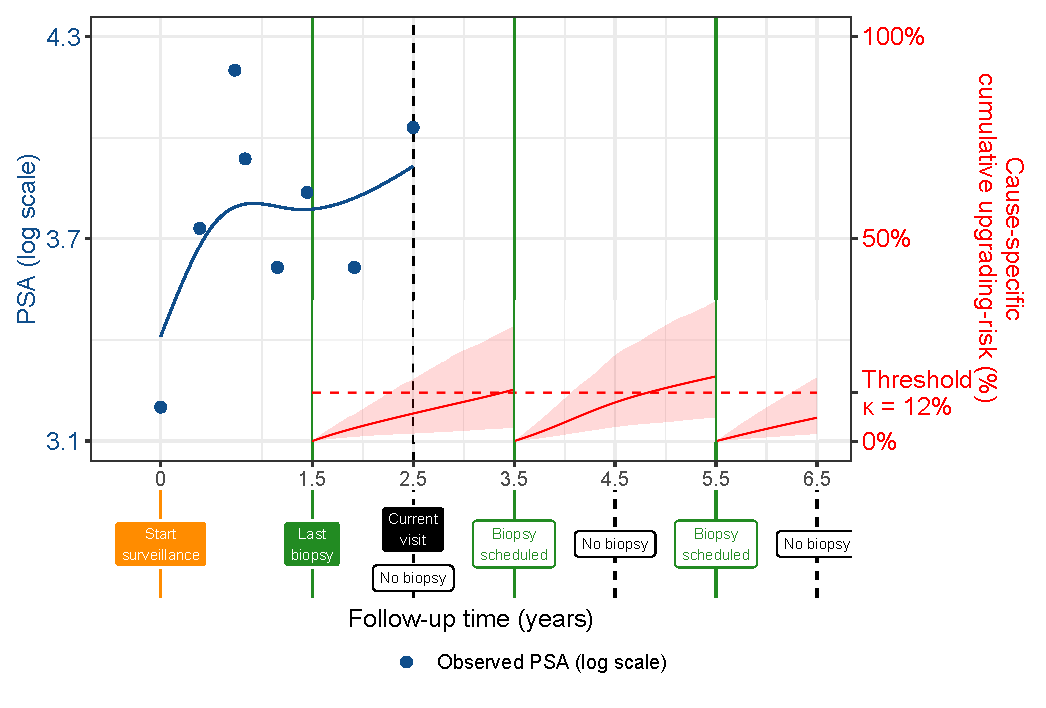
\includegraphics{images/successive_biopsy_decisions_102.eps}}
\caption{\textbf{Illustration of Personalized Biopsy Decisions Using Patient-specific Conditional Cumulative Upgrading-risk}. The last biopsy on which upgrading was not observed was conducted at $t=1.5$ years. The current visit time of the patient is $v=2.5$ years. Decisions for biopsy need to be made at a gap of every one year starting from the current visit until a horizon of 6.5 years. That is, $U=\{2.5, 3.5, 4.5, 5.5, 6.5\}$ years. Based on an example risk threshold of 12\% ($\kappa=0.12$) the future biopsy decisions at time points in $U$ lead to a personalized schedule $S_j^{\kappa^*} (U \mid t=1.5, v=2.5) = \{3.5, 5.5\}$ years. The conditional cumulative-risk profiles $R_j(u_l \mid t_l, v)$ employed in~(\ref{eq:personalized_decision_grid}) are shown with red line (confidence interval shaded). It is called `conditional' because, for example, the second biopsy at future time 5.5 years, is scheduled after accounting for the possibility that upgrading (true time $T^*_j$) may not have occurred until the time of the previously scheduled biopsy at time $T^*_j>3.5$ years. All values are illustrative.} 
\label{fig:schedule_explanation}
\end{figure}


\subsection{Expected Time Delay in Detecting Upgrading}
\label{subsec:exp_delay_estimation}
The schedule $S_j^{\kappa}(U \mid t, v)$ manifests a personalized biopsy plan for the $j$-the patient. However, the time delay in detecting upgrading that may subsequently be observed depends on the true time of upgrading $T^*_j$ of the patient. Since two different patients with the same timing of biopsies will expect different time delays, we estimate it in a patient-specific manner as well. Although, this calculation is not limited to personalized schedules only, but can be done for any schedule $S$ of biopsies with $N$ time points $S=\{s_n \mid n=1,\ldots, N\}$. 

For each of the $N$ planned biopsies there exist $N$ possible time intervals ${s_{n-1} < T^*_j \leq s_n}$ in which upgrading may be observed. Correspondingly, there are $N$ possible time delays in detecting upgrading $s_n - T^*_j$. Given a schedule $S$, the true time delay in detecting upgrading $D_j$ that the patient will experience can be defined as:
\begin{equation}
\label{eq:number_of_biopsies_and_delay}
\begin{split}
D_j (S \mid t) &= \left\{ \begin{array}{lcrr}
  s_1 - T^*_j, &\mbox{if}& t < T^*_j \leq s_1\\
  \ldots \\
  s_N - T^*_j, &\mbox{if}& s_{N-1} < T^*_j \leq s_N  
\end{array} \right\}.
\end{split}
\end{equation}
The time delay is cannot be defined for the scenario in which the patient obtains upgrading after the time of the last biopsy in the schedule $T^*_j > s_N$. Hence, this delay should be interpreted as the delay that will be observed if the patient will experience upgrading before time of the last planned biopsy at $T^*_j\leq s_N$. To estimate the expected value of $D_j(\cdot)$ in a patient-specific manner, we exploit the personalized cumulative-risk profile of the patient defined in~(\ref{eq:dynamic_risk_prob}). Specifically, the expected time delay $E\{D_j(\cdot)\}$ can be calculated as the weighted sum of $N$ possible time delays defined in~(\ref{eq:number_of_biopsies_and_delay}). The $n$-th weight is equal to the probability of the patient obtaining upgrading in the $n$-th interval ${s_{n-1} < T^*_j \leq s_n}$.
\begin{equation*}
\label{eq:expected_number_of_biopsies_and_delay}
\begin{split}
E\big\{D_j(S \mid t)\big\} &= \sum_{n=1}^{N} \Big\{s_n - E(T^*_j \mid s_{n-1}, s_n, v)\Big\} \\ & \quad \times \mbox{Pr}\Big\{s_{n-1} < T^*_j \leq s_n \mid T^*_j \leq s_N, \mathcal{Y}_j(v), \mathcal{A}_n\Big\}, \quad s_0 = t\\
E(T^*_j \mid s_{n-1}, s_n, v) &= s_{n-1} + \int_{s_{n-1}}^{s_n} \mbox{Pr}\Big\{T^*_j \geq u \mid s_{n-1} < T^*_j \leq s_n, \mathcal{Y}_{j}(v), \mathcal{A}_n\Big\} \mathrm{d}u,
\end{split}
\end{equation*}
where $E(T^*_j \mid s_{n-1}, s_n, v)$ denotes the conditional expected time of upgrading for the scenario $s_{n-1} < T^*_j \leq s_n$, and is calculated as the area under the corresponding survival curve.

The personalized expected time delay in detecting upgrading has the advantage that it is updated over follow-up as more patient data become available. Since it can be calculated for any schedule, patients and doctors can utilize it along with the plan of biopsies to compare schedules before making a decision. Although, in order to have a fair comparison of time delays between different schedules for the same patient, a compulsory biopsy at a common horizon time point should be planned in all schedules.

\begin{table}[!htb]
\small\sf\centering
\caption{\textbf{Maximum follow-up period up to which we can reliably make personalized schedules}. In each cohort, this time point is chosen such that there are at least 10 patients who experience upgrading after this time point. Full names of Cohorts are \textit{PRIAS}: Prostate Cancer International Active Surveillance, \textit{Toronto}: University of Toronto Active Surveillance, \textit{Hopkins}: Johns Hopkins Active Surveillance, \textit{MSKCC}: Memorial Sloan Kettering Cancer Center Active Surveillance, \textit{KCL}: King's College London Active Surveillance, \textit{MUSIC}: Michigan Urological Surgery Improvement Collaborative Active Surveillance, \textit{UCSF}: University of California San Francisco Active Surveillance.}
\label{tab:max_pred_time_repeat}
\begin{tabular}{l|r}
\hline
\hline
Cohort & \parbox[t]{3.75cm}{Maximum Personalized\\Schedule Time (years)}\\
\hline
PRIAS & 6\\
KCL & 3\\
MUSIC & 2\\
Toronto & 8\\
MSKCC & 6\\
Hopkins & 7\\
UCSF & 8.5\\
\hline
\end{tabular}    
\end{table}

\begin{figure}
\centerline{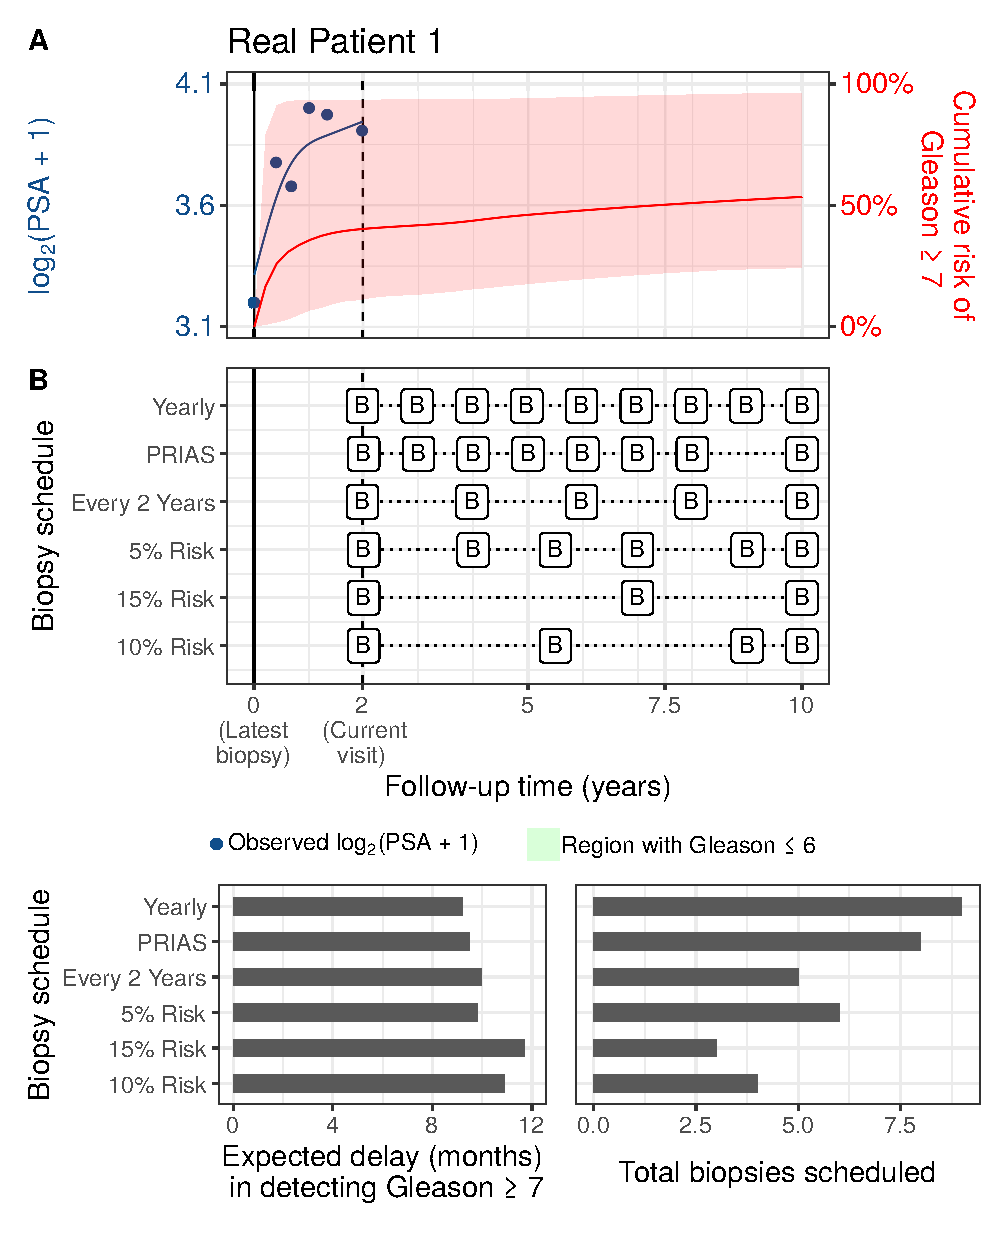
\includegraphics[width=\columnwidth]{images/demo_pat1_supp.eps}}
\caption{\textbf{Personalized and fixed schedules of biopsies for patient 1}. \textbf{Panel~A:} shows the observed and fitted $\log_2(\mbox{PSA} + 1)$ measurements (Equation~\ref{eq:long_model_psa}), and the dynamic cause-specific cumulative upgrading-risk (see \ref{sec:param_estimates_jm_fit_prias}) over follow-up period. \textbf{Panel~B} shows the personalized and fixed schedules of biopsies with a `B' indicating times of biopsies. Smaller risk thresholds lead to more frequently planned biopsies. \textbf{Panel~C} various schedules are compared in terms of the expected time delay in detecting upgrading (years) if patient progresses before year six. The maximum time delay with limited adverse consequences is three years~\citep{de2017estimating}. A compulsory biopsy was scheduled at year six (maximum biopsy scheduling time in PRIAS, Table~\ref{tab:max_pred_time_repeat}) in all schedules for a meaningful comparison between them.}
\label{fig:demo_pat1_supp}
\end{figure}

\begin{figure}
\centerline{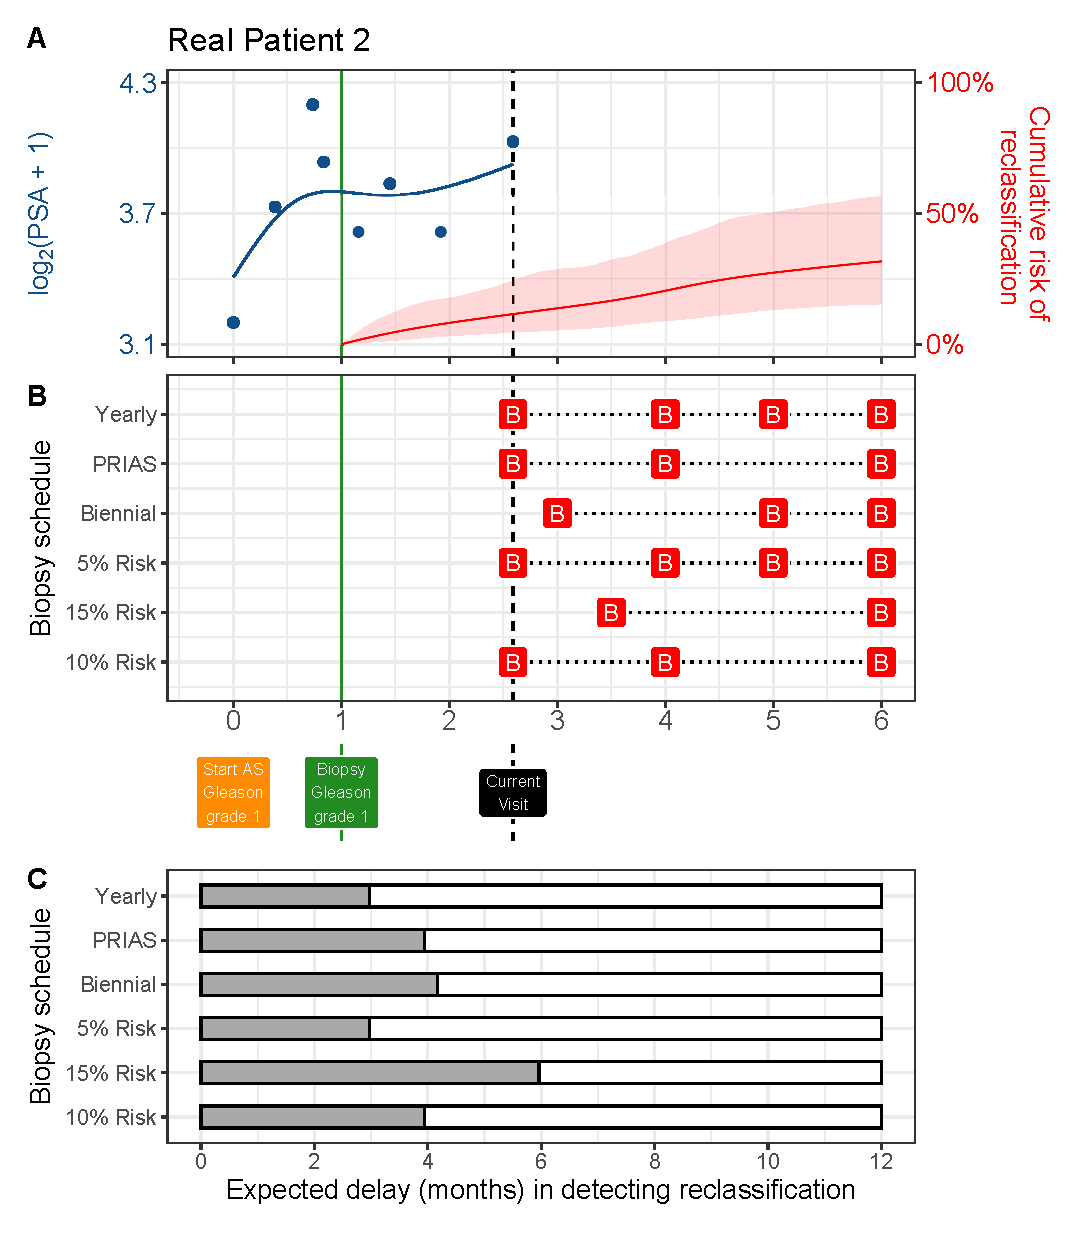
\includegraphics[width=\columnwidth]{images/demo_pat2_supp.eps}}
\caption{\textbf{Personalized and fixed schedules of biopsies for patient 2}. \textbf{Panel~A:} shows the observed and fitted $\log_2(\mbox{PSA} + 1)$ measurements (Equation~\ref{eq:long_model_psa}), and the dynamic cause-specific cumulative upgrading-risk (see \ref{sec:param_estimates_jm_fit_prias}) over follow-up period. \textbf{Panel~B} shows the personalized and fixed schedules of biopsies with a `B' indicating times of biopsies. Smaller risk thresholds lead to more frequently planned biopsies. \textbf{Panel~C} various schedules are compared in terms of the expected time delay in detecting upgrading (years) if patient progresses before year six. The maximum time delay with limited adverse consequences is three years~\citep{de2017estimating}. A compulsory biopsy was scheduled at year six (maximum biopsy scheduling time in PRIAS, Table~\ref{tab:max_pred_time_repeat}) in all schedules for a meaningful comparison between them.}
\label{fig:demo_pat2_supp}
\end{figure}

\begin{figure}
\centerline{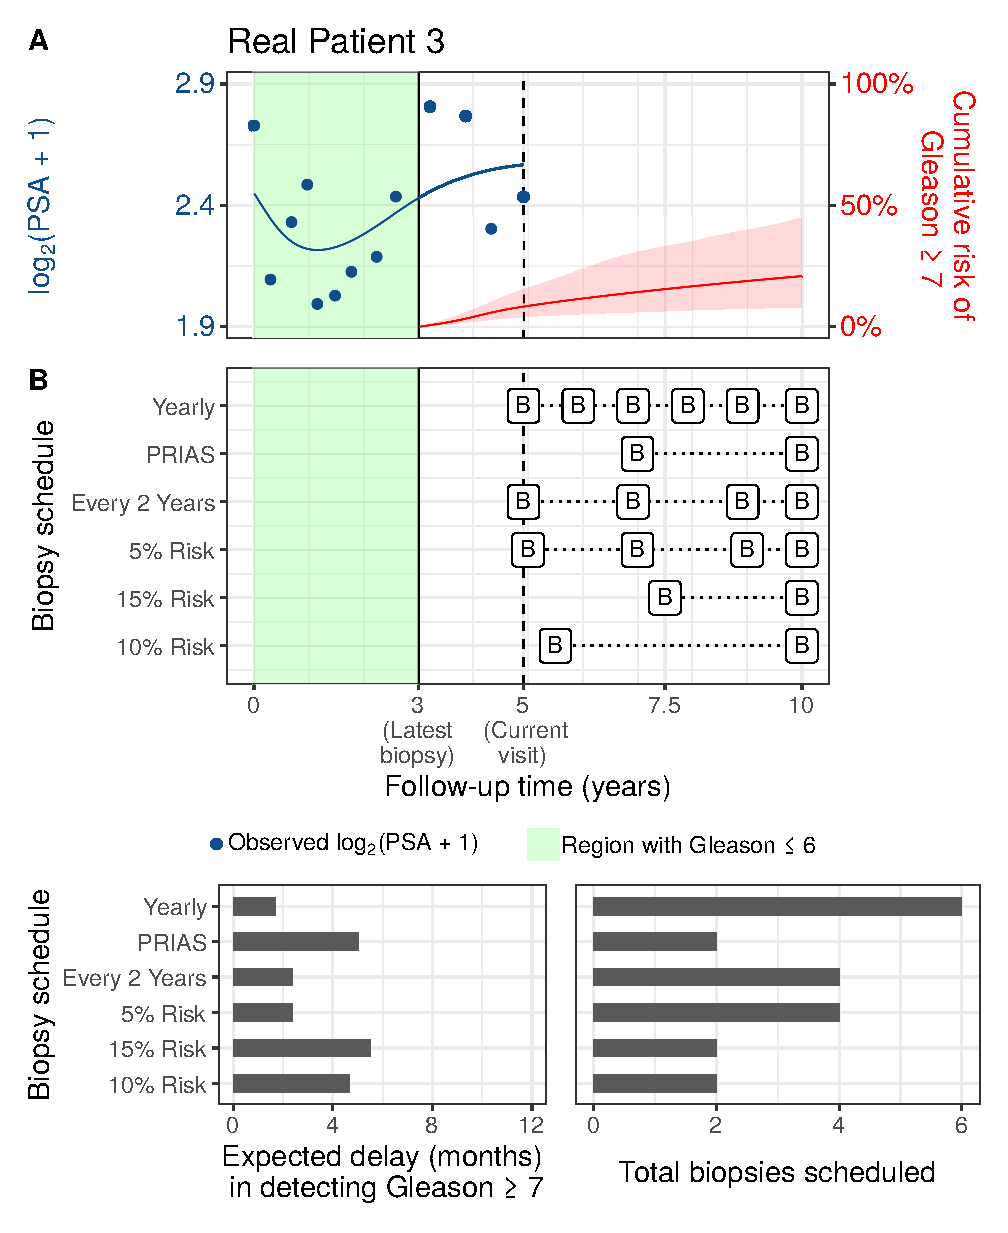
\includegraphics[width=\columnwidth]{images/demo_pat3_supp.eps}}
\caption{\textbf{Personalized and fixed schedules of biopsies for patient 3}. \textbf{Panel~A:} shows the observed and fitted $\log_2(\mbox{PSA} + 1)$ measurements (Equation~\ref{eq:long_model_psa}), and the dynamic cause-specific cumulative upgrading-risk (see \ref{sec:param_estimates_jm_fit_prias}) over follow-up period. \textbf{Panel~B} shows the personalized and fixed schedules of biopsies with a `B' indicating times of biopsies. Smaller risk thresholds lead to more frequently planned biopsies. \textbf{Panel~C} various schedules are compared in terms of the expected time delay in detecting upgrading (years) if patient progresses before year six. The maximum time delay with limited adverse consequences is three years~\citep{de2017estimating}. A compulsory biopsy was scheduled at year six (maximum biopsy scheduling time in PRIAS, Table~\ref{tab:max_pred_time_repeat}) in all schedules for a meaningful comparison between them.}
\label{fig:demo_pat3_supp}
\end{figure}